\documentclass[addpoints, 12pt]{exam}%, answers]
\usepackage[utf8]{inputenc}
\usepackage[T1]{fontenc}

\usepackage{lmodern}
\usepackage{arydshln}
\usepackage[margin=2cm]{geometry}

\usepackage{enumitem}

\usepackage{enumerate}
\usepackage{breqn}
\usepackage{parskip}

\usepackage{amsmath, amsthm, amsfonts, amssymb}
\usepackage{graphicx}
\usepackage{tikz}
\usetikzlibrary{arrows,calc,patterns}
\usepackage{pgfplots}
\pgfplotsset{compat=newest}
\usepackage{url}
\usepackage{multicol}
\usepackage{thmtools}

\usepackage{caption}
\usepackage{subcaption}

\usepackage{pifont}

% MATH commands
\newcommand{\bC}{\mathbb{C}}
\newcommand{\bR}{\mathbb{R}}
\newcommand{\bN}{\mathbb{N}}
\newcommand{\bZ}{\mathbb{Z}}
\newcommand{\bT}{\mathbb{T}}
\newcommand{\bD}{\mathbb{D}}

\DeclareMathOperator{\dom}{dom}


\newcommand{\spc}{\vspace*{0.5cm}}
\CorrectChoiceEmphasis{\color{red}}

\begin{document}
	\noindent \hrulefill \\
	MATH-241 Calculus I \hfill Created by Rukiyah Walker\\
	Homework 3 \hfill Spring 2023\\ \vspace*{-1cm}
 
	\noindent\hrulefill

\qformat{\rule{0.3\textwidth}{.4pt} \begin{large}{\textsc{Question}} \thequestion \end{large} \hspace*{0.2cm} \hrulefill \hspace*{0.1cm} \textbf{(\totalpoints\hspace*{0.1cm} pts)}}

\begin{questions}

\vspace*{1cm}

\question[1]

If $c$ is a constant and the limit $\lim_{x \to a} f(x)$ exists, then $\lim_{x \to a} [cf(x)]$ is equivalent to:
    
\begin{choices}
\choice $\lim_{x \to a} (cf(x))$
\choice $c$
\CorrectChoice $c\lim_{x \to a} f(x)$
\choice $\lim_{x \to a} (f(x)c)$
\end{choices}

\spc

\question[1]

If $\lim_{x \to a}\frac{f(x)}{g(x)} = \frac{\lim_{x \to a} f(x)}{\lim_{x \to a} g(x)}$, then:

\begin{choices}
\choice $g(x)$ = 0
\CorrectChoice $\lim_{x \to a} g(x) \neq 0$
\choice $g(x) \neq 0$
\choice $\lim_{x \to a} g(x) = 0$
\end{choices}

\question[1]

$\lim_{x \to a} [f(x)]^n$ is equivalent to:

\begin{choices}
\choice $n\lim_{x \to a} f(x)$
\choice $\lim_{x \to a} (nf(x))$
\choice $n$
\CorrectChoice $[\lim_{x \to a} f(x)]^n$
\end{choices}

\spc

\question[1]

The substitution property says: If $f$ is a polynomial or a rational function and $a$ is in the domain of $f$, then:

\begin{choices}
\choice $\lim_{x \to a} f(x) = a$
\choice $\lim_{x \to a} f(a) = f(x)$
\CorrectChoice $\lim_{x \to a} f(x) = f(a)$
\choice The limit does not exist.
\end{choices}

\newpage

\question[1]

The squeeze theorem says: If a function $g(x)$ is squeezed between two functions, $f(x)$ and $g(x)$, near a, and if $f$ and $h$ have the same limit, $L$, at $a$, then:

\begin{choices}
\CorrectChoice $g$ is forced to have the same limit, $L$, at $a$.
\choice f(x) = g(x) = h(x)
\choice $\lim_{x \to a} g(x) = f(x)$
\choice $\lim_{x \to a} g(x) = a$
\end{choices}

\spc

\question[1]

To show that a function is continuous at a number $a$, you need to verify:

\begin{choices}
\choice The function is defined at $x = a$.
\choice The limit of the function exists at $x = a$.
\choice The limit of the function at $x = a$ equals the value of the function at $x = a$.
\CorrectChoice All of the above.
\end{choices}

\spc

\question[1]

A function is discontinuous at a number $a$ if:

\begin{choices}
\CorrectChoice At least one of the criteria from question 6 is not satisfied.
\choice $f(x) = a$
\choice $L = f(a)$
\choice $\lim_{x \to a} f(x) = L$
\end{choices}

\spc

\question[1]
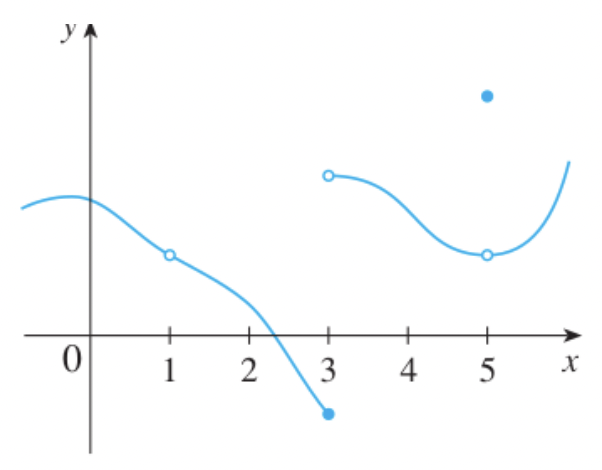
\includegraphics[width=0.3\textwidth]{Discontinuous at x.png}

At which values of $x$ is the function $f$ (graph shown above) discontinuous?

\begin{choices}
\choice When $x$ goes to $\infty$
\CorrectChoice $x = 1$, $x = 3$, and $x = 5$
\choice The function is continuous.
\choice $x = 1$
\end{choices}

\question[1]
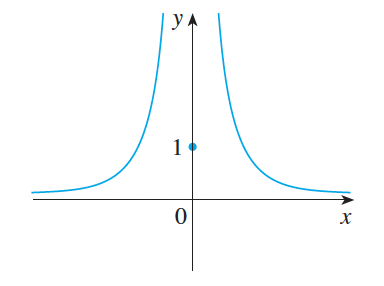
\includegraphics[width=0.3\textwidth]{Infinite discontinuity.png}

The graph above represents a function that is:

\begin{choices}
\choice Jump discontinuous.
\CorrectChoice Infinitely discontinuous.
\choice Removably discontinuous.
\choice Continuous since $f(0) = 1$.
\end{choices}

\spc

\question[1]

If $f$ is continuous at $b$ and $\lim_{x \to a} g(x) = b$, then:

\begin{choices}
\choice $f(x) = b$
\choice $g(x) = f(b)$
\CorrectChoice $\lim_{x \to a} f(g(x)) = f(\lim_{x \to a} g(x)) = f(b)$
\choice $f(b) = g(b)$
\end{choices}

\end{questions}

\end{document}